\documentclass{beamer}\usepackage[]{graphicx}\usepackage[]{color}
%% maxwidth is the original width if it is less than linewidth
%% otherwise use linewidth (to make sure the graphics do not exceed the margin)
\makeatletter
\def\maxwidth{ %
  \ifdim\Gin@nat@width>\linewidth
    \linewidth
  \else
    \Gin@nat@width
  \fi
}
\makeatother

\definecolor{fgcolor}{rgb}{0.345, 0.345, 0.345}
\newcommand{\hlnum}[1]{\textcolor[rgb]{0.686,0.059,0.569}{#1}}%
\newcommand{\hlstr}[1]{\textcolor[rgb]{0.192,0.494,0.8}{#1}}%
\newcommand{\hlcom}[1]{\textcolor[rgb]{0.678,0.584,0.686}{\textit{#1}}}%
\newcommand{\hlopt}[1]{\textcolor[rgb]{0,0,0}{#1}}%
\newcommand{\hlstd}[1]{\textcolor[rgb]{0.345,0.345,0.345}{#1}}%
\newcommand{\hlkwa}[1]{\textcolor[rgb]{0.161,0.373,0.58}{\textbf{#1}}}%
\newcommand{\hlkwb}[1]{\textcolor[rgb]{0.69,0.353,0.396}{#1}}%
\newcommand{\hlkwc}[1]{\textcolor[rgb]{0.333,0.667,0.333}{#1}}%
\newcommand{\hlkwd}[1]{\textcolor[rgb]{0.737,0.353,0.396}{\textbf{#1}}}%
\let\hlipl\hlkwb

\usepackage{framed}
\makeatletter
\newenvironment{kframe}{%
 \def\at@end@of@kframe{}%
 \ifinner\ifhmode%
  \def\at@end@of@kframe{\end{minipage}}%
  \begin{minipage}{\columnwidth}%
 \fi\fi%
 \def\FrameCommand##1{\hskip\@totalleftmargin \hskip-\fboxsep
 \colorbox{shadecolor}{##1}\hskip-\fboxsep
     % There is no \\@totalrightmargin, so:
     \hskip-\linewidth \hskip-\@totalleftmargin \hskip\columnwidth}%
 \MakeFramed {\advance\hsize-\width
   \@totalleftmargin\z@ \linewidth\hsize
   \@setminipage}}%
 {\par\unskip\endMakeFramed%
 \at@end@of@kframe}
\makeatother

\definecolor{shadecolor}{rgb}{.97, .97, .97}
\definecolor{messagecolor}{rgb}{0, 0, 0}
\definecolor{warningcolor}{rgb}{1, 0, 1}
\definecolor{errorcolor}{rgb}{1, 0, 0}
\newenvironment{knitrout}{}{} % an empty environment to be redefined in TeX

\usepackage{alltt}
\newenvironment{changemargin}[2]{%
\begin{list}{}{%
\setlength{\topsep}{0pt}%
\setlength{\leftmargin}{#1}%
\setlength{\rightmargin}{#2}%
\setlength{\listparindent}{\parindent}%
\setlength{\itemindent}{\parindent}%
\setlength{\parsep}{\parskip}%
}%
\item[]}{\end{list}}
\usepackage{graphicx}
\usepackage{amsmath}
\usepackage{url}
\usepackage{grffile}
\usetheme{Madrid}
\usecolortheme{beaver}
\setbeamertemplate{navigation symbols}{}
\titlegraphic{
\includegraphics[width=5cm]{..//..//S-DS-VC-RGB.png}\hspace*{1cm}~%
   
\includegraphics[width=5cm]{..//..//CompassLogo.jpg}
}
%\logo{
\includegraphics[width=0.1\textwidth,keepaspectratio]{..//..//UOACrest.png}}
\author[SCC]{Statistical Consulting Centre}%\\
\institute[\href{mailto:consulting@stat.auckland.ac.nz}
  {consulting@stat.auckland.ac.nz}]{\href{mailto:consulting@stat.auckland.ac.nz}
  {consulting@stat.auckland.ac.nz}\\
  k.chang@auckland.ac.nz\\
%Statistical Consulting Centre\\
The Department of Statistics\\
The University of Auckland}
\title[Session 8 -- Advanced analysis]{NZSSN Courses: Introduction
to \texttt{R}}
\subtitle{Session 8 -- Advanced analysis}
\date{2 March, 2017}
\IfFileExists{upquote.sty}{\usepackage{upquote}}{}
\begin{document}
%\SweaveOpts{concordance=TRUE}
\maketitle
 
\begin{frame}[fragile]
  \frametitle{Linear regression}

\verb|lm(y~x)| is used for linear regression.
  \begin{itemize}
  \item \texttt{y}, the response variable.
  \item \texttt{x}, the explanatory variable.   
  \item There can be more than one explanatory variable, called {\em multiple} linear regression. 
  \item Both response variable and explanatory variable(s) should be numeric, it is {\em generalised} linear regression.
  \end{itemize}
\end{frame} 

\begin{frame}[fragile]
\frametitle{Simple linear regression}
When there is only one predictor variable (e.g. Age) in our linear regression, we refer to this as {\em simple} linear regression.
\begin{knitrout}
\definecolor{shadecolor}{rgb}{0.969, 0.969, 0.969}\color{fgcolor}

{\centering 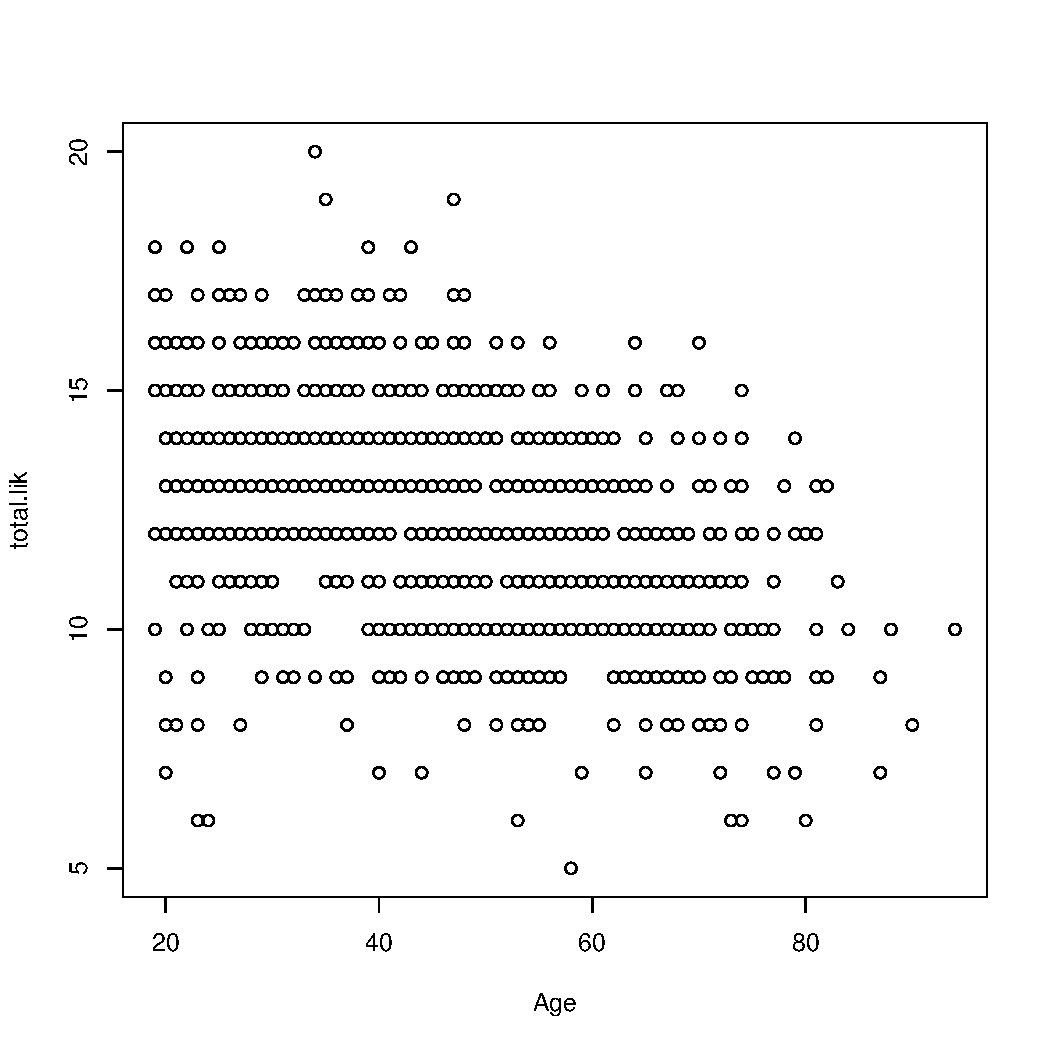
\includegraphics[width=0.6\linewidth]{figure/unnamed-chunk-2-1} 

}



\end{knitrout}
\end{frame} 

\begin{frame}[fragile]
\frametitle{Simple linear regression}
\begin{itemize}
 \item The relationship between age and total score appears weakly negative, i.e. total score decreases with age.
 \item Let's carry out the linear regression of Age on total score, i.e.
\begin{knitrout}
\definecolor{shadecolor}{rgb}{0.969, 0.969, 0.969}\color{fgcolor}\begin{kframe}
\begin{alltt}
\hlstd{try.lm} \hlkwb{<-} \hlkwd{with}\hlstd{(issp.df,} \hlkwd{lm}\hlstd{(total.lik}\hlopt{~}\hlstd{Age))}
\end{alltt}
\end{kframe}
\end{knitrout}
\end{itemize}
\end{frame} 

\begin{frame}[fragile]
\frametitle{Simple linear regression}
\begin{scriptsize}
\begin{knitrout}
\definecolor{shadecolor}{rgb}{0.969, 0.969, 0.969}\color{fgcolor}\begin{kframe}
\begin{alltt}
\hlkwd{summary}\hlstd{(try.lm)}
\end{alltt}
\begin{verbatim}

Call:
lm(formula = total.lik ~ Age)

Residuals:
    Min      1Q  Median      3Q     Max 
-7.7897 -1.2829  0.0273  1.3692  6.8813 

Coefficients:
             Estimate Std. Error t value Pr(>|t|)    
(Intercept) 15.192553   0.200219   75.88   <2e-16 ***
Age         -0.060995   0.004173  -14.62   <2e-16 ***
---
Signif. codes:  0 '***' 0.001 '**' 0.01 '*' 0.05 '.' 0.1 ' ' 1

Residual standard error: 2.082 on 952 degrees of freedom
  (93 observations deleted due to missingness)
Multiple R-squared:  0.1833,	Adjusted R-squared:  0.1824 
F-statistic: 213.6 on 1 and 952 DF,  p-value: < 2.2e-16
\end{verbatim}
\end{kframe}
\end{knitrout}
\end{scriptsize}
\end{frame} 


\begin{frame}[fragile]
\frametitle{Simple linear regression}
\begin{knitrout}
\definecolor{shadecolor}{rgb}{0.969, 0.969, 0.969}\color{fgcolor}\begin{kframe}
\begin{verbatim}
               Estimate  Std. Error   t value     Pr(>|t|)
(Intercept) 15.19255299 0.200218824  75.87974 0.000000e+00
Age         -0.06099486 0.004173331 -14.61539 8.528271e-44
\end{verbatim}
\end{kframe}
\end{knitrout}
\begin{itemize}
\item The estimated intercept is 15.19. There is very strong evidence that this is not zero ($p$-value $< 0.0001$).
\item The estimated slope is -0.06. There is very strong evidence that this is not zero ($p$-value $< 0.0001$).
\item The fitted line is \texttt{total.lik} = -0.06 $\times$ \texttt{Age} + 15.19
\item For every one year increase in age, the mean total score decreases by 0.06 units on the likert scale.
\end{itemize}
\end{frame} 

\begin{frame}[fragile]
\frametitle{Check the fit: Residual plots}
\begin{knitrout}
\definecolor{shadecolor}{rgb}{0.969, 0.969, 0.969}\color{fgcolor}\begin{kframe}
\begin{alltt}
\hlkwd{plot}\hlstd{(}\hlkwd{residuals}\hlstd{(try.lm))}
\end{alltt}
\end{kframe}

{\centering 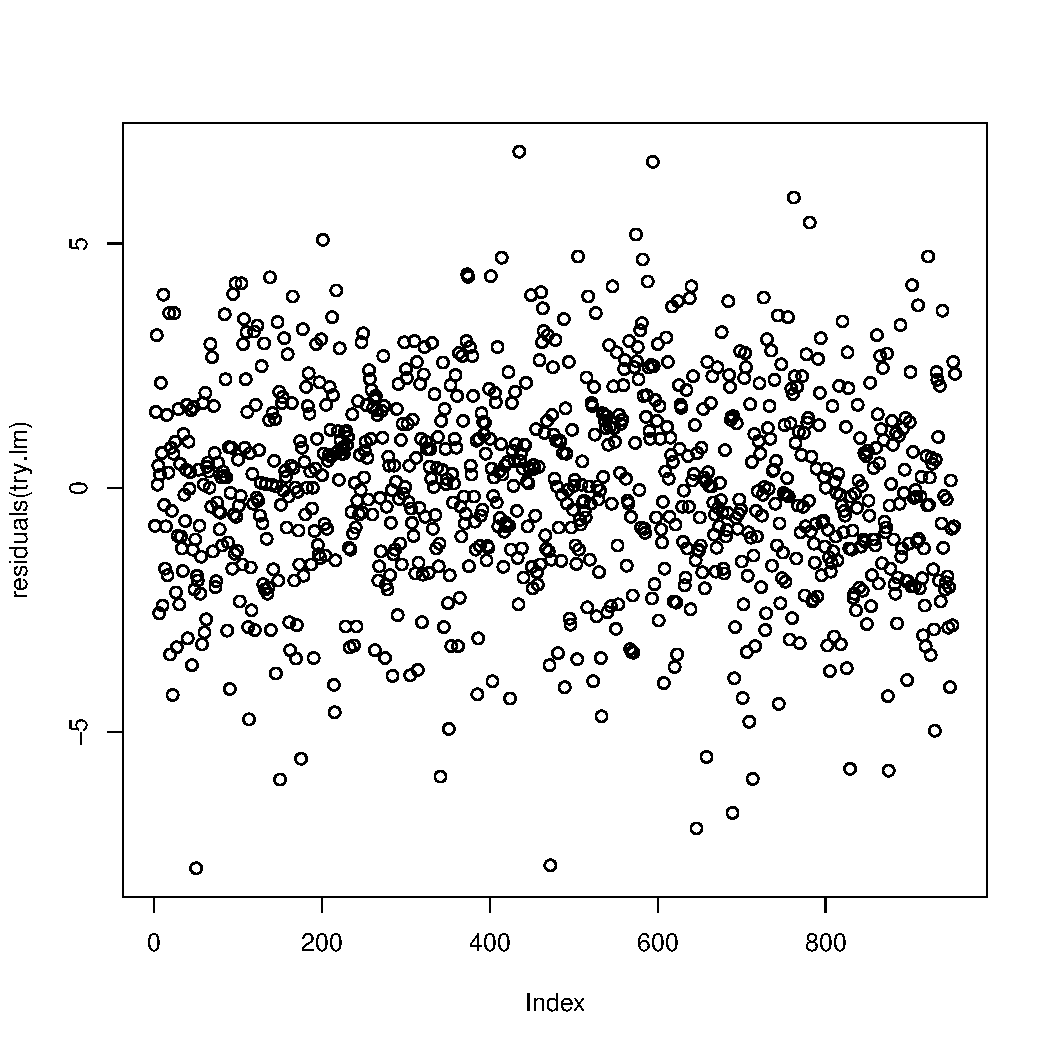
\includegraphics[width=0.6\linewidth]{figure/unnamed-chunk-6-1} 

}



\end{knitrout}
\end{frame} 

\begin{frame}[fragile]
\frametitle{Are the residuals approximately normal?}
\begin{knitrout}
\definecolor{shadecolor}{rgb}{0.969, 0.969, 0.969}\color{fgcolor}\begin{kframe}
\begin{alltt}
\hlkwd{qqnorm}\hlstd{(}\hlkwd{residuals}\hlstd{(try.lm))}
\hlkwd{qqline}\hlstd{(}\hlkwd{residuals}\hlstd{(try.lm),} \hlkwc{col} \hlstd{=} \hlnum{2}\hlstd{,} \hlkwc{lwd} \hlstd{=} \hlnum{2}\hlstd{)}
\end{alltt}
\end{kframe}

{\centering 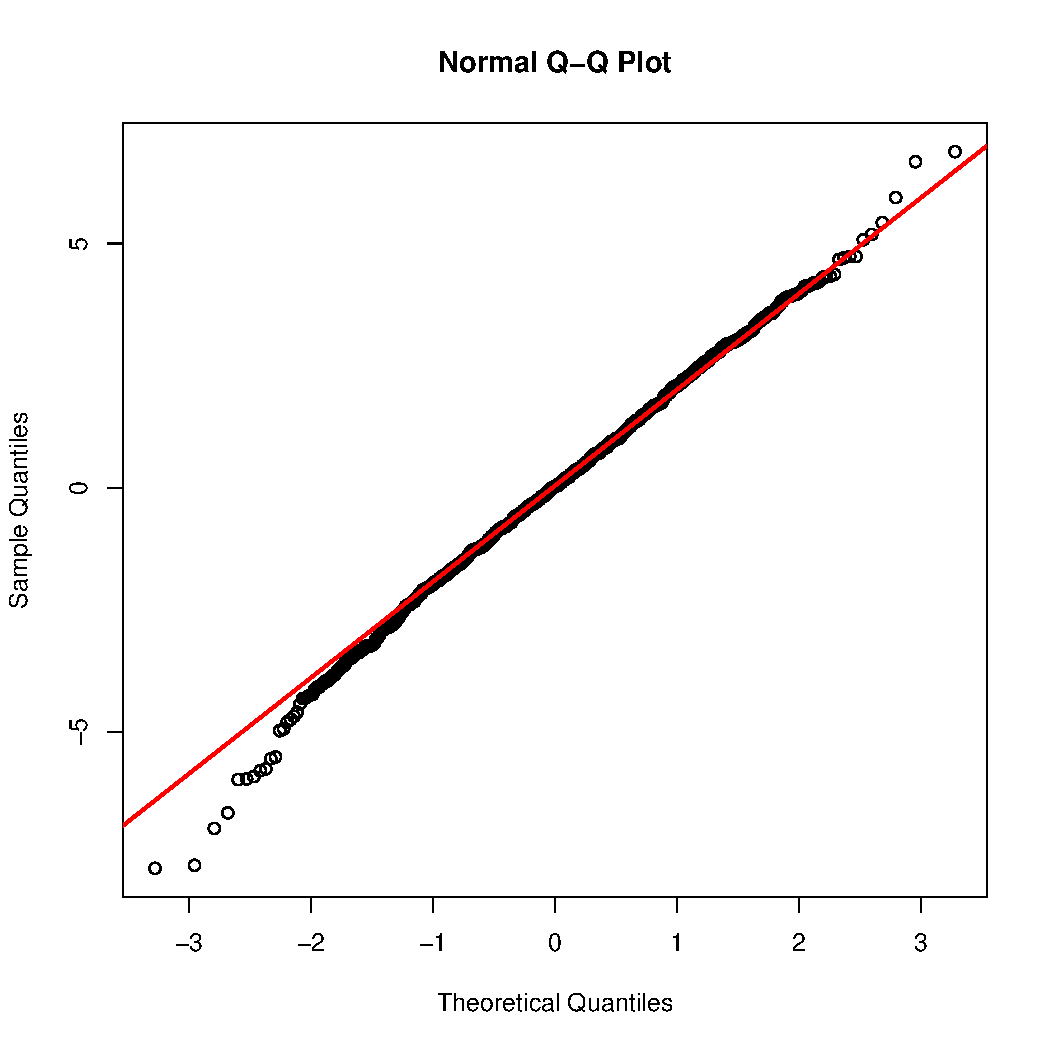
\includegraphics[width=0.6\linewidth]{figure/unnamed-chunk-7-1} 

}



\end{knitrout}
\end{frame} 


\begin{frame}[fragile]
\frametitle{Conclusion}
\begin{itemize}
\item The linear relationship between age and total score is statistically significant.
\item Total score is negatively related to age.
\end{itemize}
\end{frame}


\begin{frame}[fragile]
  \frametitle{Add the fitted line}
\begin{knitrout}
\definecolor{shadecolor}{rgb}{0.969, 0.969, 0.969}\color{fgcolor}\begin{kframe}
\begin{alltt}
\hlkwd{with}\hlstd{(issp.df,} \hlkwd{plot}\hlstd{(Age, total.lik))}
\hlkwd{abline}\hlstd{(try.lm,} \hlkwc{col} \hlstd{=} \hlnum{2}\hlstd{)}
\end{alltt}
\end{kframe}
\end{knitrout}

\begin{figure}[h]
  \vspace{-20pt}
  \centering
  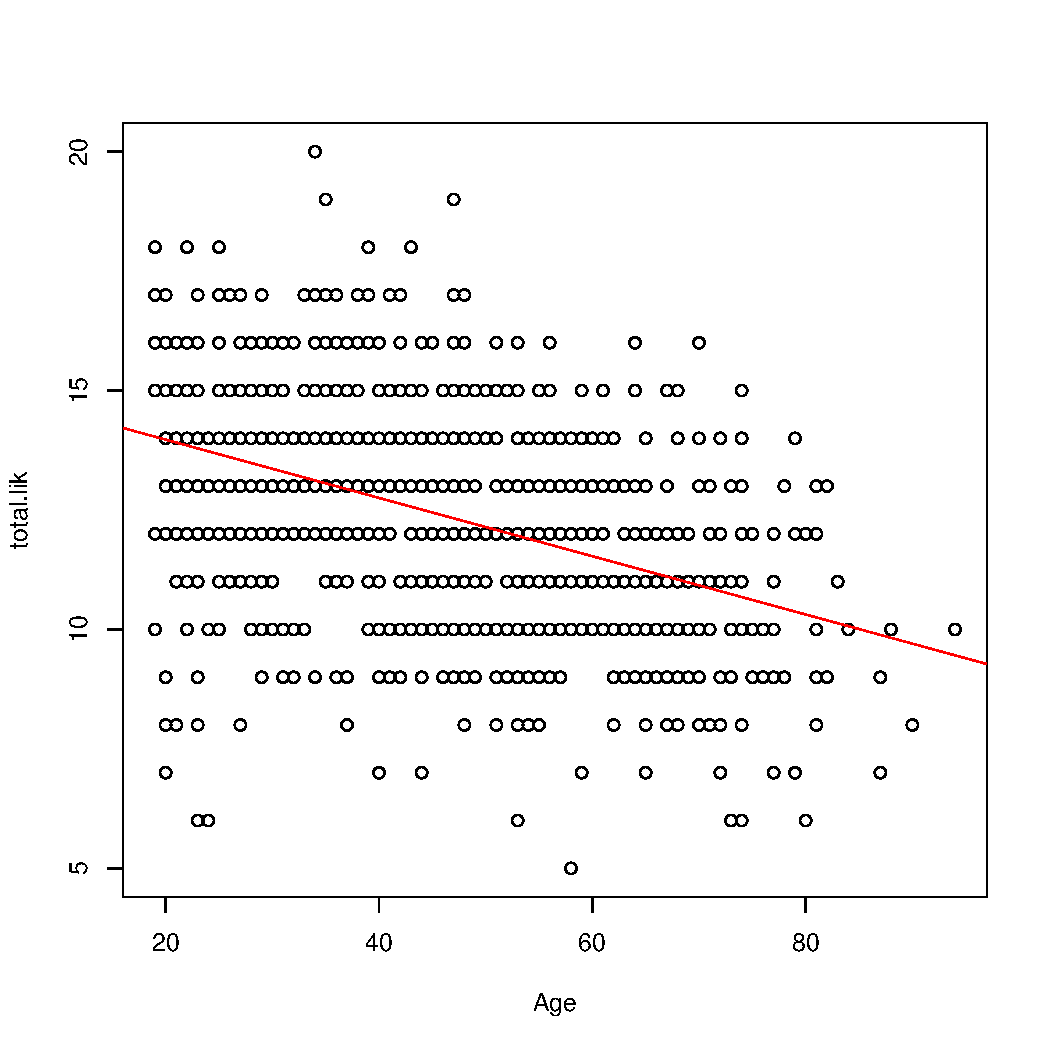
\includegraphics[height = 0.6\textwidth, keepaspectratio]{Figure/fitted}
  %\vspace{-20pt}
  %\caption{Boxplots of PM10 in 2006--2012}
  \label{fig:fitted}
\end{figure}
\end{frame} 

\begin{frame}[fragile]
\frametitle{What if the response variable is \emph{not} continuous?}
So far, we have considered methods for analysing response variables 
measured on a continuous scale.\\
\vspace{0.2cm}
Often, measurements are:
  \begin{itemize}
\item \emph{Counts} per unit time, e.g. number of hours worked in a working week.
\item \emph{Binary} responses, e.g. Gender.
\item \emph{Generalised} linear models: \emph{Poisson} (counts) and \emph{Logistic} (binary) regression
\item \emph{Today} logistic regression \emph{only}
\end{itemize}
\end{frame}

\begin{frame}[fragile]
\frametitle{Logistic regression}
\begin{itemize}
\item Relates a \textcolor{blue}{\emph{binary}} \emph{response variable}
to a continuous and/or categorical variable
\item Let's illustrate by example using \texttt{issp.df}.
\begin{itemize}
\item Consider the variable \texttt{Q5} with values `\texttt{be obedient}' and '\texttt{think themselves}'.
\end{itemize}
\end{itemize}
\end{frame}

\begin{frame}[fragile]
\frametitle{Logistic regression}
\begin{center}
\textbf{Question} \\
Is \texttt{Age} a useful indicator of choosing `\texttt{being obedient}' as important in preparing for children for life? \\[0.2cm]
\textbf{How do we answer this?} \\
By relating the \emph{probability} of \texttt{being obedient} 
to \texttt{Age}.
\end{center}  
\begin{itemize}
\item Linear regression is \emph{not} suitable here because:
\begin{itemize}
\item It assumes the response variable (\texttt{Q5}) takes values from $-\infty$ to $+\infty$.\\
\item But \texttt{Q5} takes only two values, namely \texttt{being obedient} or \texttt{think themselves}!
\end{itemize}
\end{itemize}
\end{frame}

\begin{frame}[fragile]
\frametitle{Relating a probability to an explanatory variable}
Let:
\begin{itemize}
  \item $p = \Pr\left(\mathtt{Q5} = \mathtt{being}\mbox{ }\mathtt{obedient} \right)$
  \item $1-p = \Pr\left(\mathtt{Q5} = \mathtt{think}\mbox{ }\mathtt{themselves} \right)$
\end{itemize}
\vspace{0.2cm}
\textbf{Definition:} The \emph{odds} that a respondent of \texttt{Q5} chooses \texttt{being\mbox{ }obedient} is
\[ \text{odds} = \frac{p}{1-p}. \]
\begin{itemize}
\item The \emph{odds} of an event (i.e.  $\mathtt{Q5} = \mathtt{being}\mbox{ } \mathtt{obedient}$) 
tells us how likely that event is to occur relative to it not
occurring.
\item To relate $p$ to an explanatory variable, we need the \textbf{\emph{log-odds}}, i.e.
\end{itemize}
\[ \log\left(\frac{p}{1-p}\right) = \mathtt{Intercept} + \mathtt{Slope} \times \mathtt{Age}. \]
\begin{itemize}
\item $\log\left(\frac{p}{1-p}\right)$ is known as the \emph{logit} transformation
\end{itemize}
\end{frame}



\begin{frame}[fragile]
\frametitle{GLMs in \texttt{R}: \texttt{glm()}}
\texttt{glm(formula, family, ...)}
\begin{itemize}
\item \texttt{formula:} Similar format as \texttt{lm()}; response
variable and explanatory variable(s) separated by \verb|~|.
\item \texttt{family:} Use \texttt{family = binomial} for logistic
regression.
\item \texttt{...} See the help file of \texttt{glm} (\texttt{?glm})
for other arguments.
\end{itemize}
%By default, \texttt{R} chooses the highest level as the response
\end{frame}


\begin{frame}[fragile]
\frametitle{Logistic regression: Example}
Suppose we want to find out whether older people are more likely to consider {\em being obedient} as more important in preparing children for life than is {\em thinking for themselves}.\\\vspace{0.5cm}

Statisically speaking, we want to test whether the probability of choosing ``\texttt{be obedient}'' in \texttt{Q5} increases/decreases/does not change with \texttt{Age}.
\end{frame}


\begin{frame}[fragile]
\frametitle{Logistic regression: Example}
\begin{itemize}
  \item Declare the response variable \texttt{Q5} as a integer/numeric.
  \item \texttt{be obedient} is assigned the numeric value 1 and 
        \texttt{think themselves} is assigned numeric value 0.
  \item It follows, therefore, that:
  \begin{enumerate}    
    \item $p=\Pr(\mathtt{be\mbox{ }obedient})$
    \item $p/(1-p)$ is the odds of participants selecting 
          ``being obedient'' relative to selecting 
          ``thinking for themselves'' as being important in preparing
          children for life.
  \end{enumerate}
\end{itemize}
Note: Here, the explanatory variable Age is integer/numeric.
\end{frame}


\begin{frame}[fragile]
\frametitle{GLMs in \texttt{R}: \texttt{glm()}}
\begin{knitrout}
\definecolor{shadecolor}{rgb}{0.969, 0.969, 0.969}\color{fgcolor}\begin{kframe}
\begin{alltt}
\hlcom{## class of Q5?}
\hlkwd{class}\hlstd{(issp.df}\hlopt{$}\hlstd{Q5)}
\end{alltt}
\begin{verbatim}
[1] "character"
\end{verbatim}
\begin{alltt}
\hlcom{## Convert Q5 to a variable of type 'numeric'}
\hlstd{issp.df}\hlopt{$}\hlstd{Q5} \hlkwb{<-} \hlkwd{ifelse}\hlstd{(issp.df}\hlopt{$}\hlstd{Q5} \hlopt{==} \hlstr{"be obedient"}\hlstd{,} \hlnum{1}\hlstd{,} \hlnum{0}\hlstd{)}

\hlcom{## Numeric values of Q5?}
\hlkwd{class}\hlstd{(issp.df}\hlopt{$}\hlstd{Q5)}
\end{alltt}
\begin{verbatim}
[1] "numeric"
\end{verbatim}
\end{kframe}
\end{knitrout}
\end{frame}


\begin{frame}[fragile]
\frametitle{Logistic regression: Example}
Fit the model with \texttt{glm()}
\vspace{-2mm}
\begin{knitrout}
\definecolor{shadecolor}{rgb}{0.969, 0.969, 0.969}\color{fgcolor}\begin{kframe}
\begin{alltt}
\hlstd{try.glm} \hlkwb{<-} \hlkwd{with}\hlstd{(issp.df,} \hlkwd{glm}\hlstd{(Q5}\hlopt{~}\hlstd{Age,}
                             \hlkwc{family} \hlstd{= binomial))}
\end{alltt}
\end{kframe}
\end{knitrout}
\begin{itemize}
\item \texttt{family = binomial}, logistic regression.
\end{itemize}
\vspace{-2mm}
\begin{scriptsize}
\begin{knitrout}
\definecolor{shadecolor}{rgb}{0.969, 0.969, 0.969}\color{fgcolor}\begin{kframe}
\begin{alltt}
\hlkwd{summary}\hlstd{(try.glm)}
\end{alltt}
\end{kframe}
\end{knitrout}
\end{scriptsize}
\vspace{-5mm}
\begin{scriptsize}
\begin{knitrout}
\definecolor{shadecolor}{rgb}{0.969, 0.969, 0.969}\color{fgcolor}\begin{kframe}
\begin{verbatim}

Call:
glm(formula = Q5 ~ Age, family = binomial)

Deviance Residuals: 
    Min       1Q   Median       3Q      Max  
-1.2024  -0.7108  -0.5462  -0.4299   2.2182  

Coefficients:
             Estimate Std. Error z value Pr(>|z|)    
(Intercept) -3.132552   0.278107 -11.264  < 2e-16 ***
Age          0.036263   0.005163   7.024 2.16e-12 ***
---
Signif. codes:  0 '***' 0.001 '**' 0.01 '*' 0.05 '.' 0.1 ' ' 1

(Dispersion parameter for binomial family taken to be 1)

    Null deviance: 929.45  on 920  degrees of freedom
Residual deviance: 877.21  on 919  degrees of freedom
  (126 observations deleted due to missingness)
AIC: 881.21

Number of Fisher Scoring iterations: 4
\end{verbatim}
\end{kframe}
\end{knitrout}
\end{scriptsize}
\end{frame}

\begin{frame}[fragile]
\frametitle{Logistic regression: Example}
\begin{knitrout}
\definecolor{shadecolor}{rgb}{0.969, 0.969, 0.969}\color{fgcolor}\begin{kframe}
\begin{verbatim}
               Estimate  Std. Error    z value     Pr(>|z|)
(Intercept) -3.13255166 0.278106937 -11.263839 1.979445e-29
Age          0.03626334 0.005162854   7.023894 2.157690e-12
\end{verbatim}
\end{kframe}
\end{knitrout}
\begin{eqnarray*}
\text{logit}(\text{be obedient}) & = & -3.13 + 0.04 \times \text{Age}.\\
\text{Odds}(\text{be obedient}) & = & e^{-3.13 + 0.04 \times \text{Age}}\\
\text{Probability}(\text{be obedient}) & = & \frac{e^{-3.13 + 0.04 \times \text{Age}}}{1 + e^{-3.13 + 0.04 \times \text{Age}}}
\end{eqnarray*}
\end{frame}

\begin{frame}[fragile]
\frametitle{Prediction from the model}
\begin{knitrout}
\definecolor{shadecolor}{rgb}{0.969, 0.969, 0.969}\color{fgcolor}\begin{kframe}
\begin{alltt}
\hlcom{# Logit scale, usually referred to as the }
\hlcom{# 'linear predictor' scale}
\hlstd{lp} \hlkwb{<-} \hlkwd{predict}\hlstd{(try.glm,} \hlkwd{data.frame}\hlstd{(}\hlkwc{Age} \hlstd{=} \hlnum{50}\hlstd{))}
\hlstd{lp}
\end{alltt}
\begin{verbatim}
        1 
-1.319385 
\end{verbatim}
\begin{alltt}
\hlcom{# Calculate the odds}
\hlkwd{exp}\hlstd{(lp)}
\end{alltt}
\begin{verbatim}
        1 
0.2672997 
\end{verbatim}
\end{kframe}
\end{knitrout}
Interpretation: A 50-year old is \textbf{0.3 times} likely to consider {\em being obedient} important preparation for life than {\em thinking for oneself}. Or, a 50-year old is \textbf{3.7 times more} likely to {\em thinking for oneself} than {\em being obedient}.
\end{frame}

\begin{frame}[fragile]
\frametitle{Prediction from the model}
\begin{knitrout}
\definecolor{shadecolor}{rgb}{0.969, 0.969, 0.969}\color{fgcolor}\begin{kframe}
\begin{alltt}
\hlcom{#Probability scale}
\hlkwd{predict}\hlstd{(try.glm,} \hlkwd{data.frame}\hlstd{(}\hlkwc{Age} \hlstd{=} \hlnum{50}\hlstd{),} \hlkwc{type} \hlstd{=} \hlstr{"response"}\hlstd{)}
\end{alltt}
\begin{verbatim}
        1 
0.2109207 
\end{verbatim}
\end{kframe}
\end{knitrout}
Interpretation: The probability that a 50-year old considers {\em being obedient} important preparation for life is 0.2109207.
\end{frame}

\begin{frame}[fragile]
\frametitle{Putting prediction into context}
\begin{knitrout}
\definecolor{shadecolor}{rgb}{0.969, 0.969, 0.969}\color{fgcolor}\begin{kframe}
\begin{alltt}
\hlcom{#Probability with standard error}
\hlkwd{predict}\hlstd{(try.glm,} \hlkwd{data.frame}\hlstd{(}\hlkwc{Age} \hlstd{=} \hlnum{50}\hlstd{),}
\hlkwc{type} \hlstd{=} \hlstr{"response"}\hlstd{,} \hlkwc{se.fit} \hlstd{=} \hlnum{TRUE}\hlstd{)}
\end{alltt}
\begin{verbatim}
$fit
        1 
0.2109207 

$se.fit
         1 
0.01409851 

$residual.scale
[1] 1
\end{verbatim}
\end{kframe}
\end{knitrout}
\end{frame}

\begin{frame}[fragile]
\frametitle{Categorical explanatory variables}
\begin{scriptsize}
\begin{knitrout}
\definecolor{shadecolor}{rgb}{0.969, 0.969, 0.969}\color{fgcolor}\begin{kframe}
\begin{alltt}
\hlstd{try.glm2} \hlkwb{<-} \hlkwd{with}\hlstd{(issp.df,} \hlkwd{glm}\hlstd{(Q5}\hlopt{~}\hlstd{age.group,} \hlkwc{family} \hlstd{= binomial))}
\hlkwd{anova}\hlstd{(try.glm2,} \hlkwc{test} \hlstd{=} \hlstr{"Chisq"}\hlstd{)}
\end{alltt}
\begin{verbatim}
Analysis of Deviance Table

Model: binomial, link: logit

Response: Q5

Terms added sequentially (first to last)


          Df Deviance Resid. Df Resid. Dev  Pr(>Chi)    
NULL                        920     929.45              
age.group  2   46.725       918     882.73 7.143e-11 ***
---
Signif. codes:  0 '***' 0.001 '**' 0.01 '*' 0.05 '.' 0.1 ' ' 1
\end{verbatim}
\end{kframe}
\end{knitrout}
\end{scriptsize}
Analysis of deviance table for a \texttt{glm()} object (generated using \texttt{anova()}) is analogous to ANOVA table for an \texttt{lm()} object.
\end{frame}


\begin{frame}[fragile]
\frametitle{Categorical explanatory variables}
\begin{scriptsize}
\begin{knitrout}
\definecolor{shadecolor}{rgb}{0.969, 0.969, 0.969}\color{fgcolor}\begin{kframe}
\begin{alltt}
\hlkwd{anova}\hlstd{(try.glm2,} \hlkwc{test} \hlstd{=} \hlstr{"Chisq"}\hlstd{)}
\end{alltt}
\begin{verbatim}
Analysis of Deviance Table

Model: binomial, link: logit

Response: Q5

Terms added sequentially (first to last)


          Df Deviance Resid. Df Resid. Dev  Pr(>Chi)    
NULL                        920     929.45              
age.group  2   46.725       918     882.73 7.143e-11 ***
---
Signif. codes:  0 '***' 0.001 '**' 0.01 '*' 0.05 '.' 0.1 ' ' 1
\end{verbatim}
\end{kframe}
\end{knitrout}
\end{scriptsize}
We have extremely strong evidence that at least one age group has different log-odds of choosing "be obedient" from the other age groups.
\end{frame}


\begin{frame}[fragile]
\frametitle{Categorical explanatory variables}
\begin{scriptsize}
\begin{knitrout}
\definecolor{shadecolor}{rgb}{0.969, 0.969, 0.969}\color{fgcolor}\begin{kframe}
\begin{alltt}
\hlkwd{summary}\hlstd{(try.glm2)}
\end{alltt}
\begin{verbatim}

Call:
glm(formula = Q5 ~ age.group, family = binomial)

Deviance Residuals: 
    Min       1Q   Median       3Q      Max  
-0.9790  -0.6169  -0.6169  -0.5233   2.0279  

Coefficients:
                  Estimate Std. Error z value Pr(>|z|)    
(Intercept)        -1.9192     0.1737 -11.048  < 2e-16 ***
age.group36 to 60   0.3568     0.2157   1.654    0.098 .  
age.groupOver 61    1.4327     0.2274   6.301 2.96e-10 ***
---
Signif. codes:  0 '***' 0.001 '**' 0.01 '*' 0.05 '.' 0.1 ' ' 1

(Dispersion parameter for binomial family taken to be 1)

    Null deviance: 929.45  on 920  degrees of freedom
Residual deviance: 882.73  on 918  degrees of freedom
  (126 observations deleted due to missingness)
AIC: 888.73

Number of Fisher Scoring iterations: 4
\end{verbatim}
\end{kframe}
\end{knitrout}
\end{scriptsize}
\end{frame}


\begin{frame}[fragile]
\frametitle{Categorical explanatory variables}
\begin{knitrout}\small
\definecolor{shadecolor}{rgb}{0.969, 0.969, 0.969}\color{fgcolor}\begin{kframe}
\begin{verbatim}
                    Estimate Std. Error    z value     Pr(>|z|)
(Intercept)       -1.9192419  0.1737143 -11.048269 2.234812e-28
age.group36 to 60  0.3568389  0.2156919   1.654392 9.804798e-02
age.groupOver 61   1.4327090  0.2273911   6.300639 2.964214e-10
\end{verbatim}
\end{kframe}
\end{knitrout}
\begin{itemize}
  \item \texttt{(Intercept)} corresponds to the reference age group, namely
  ``Under 35'' which is the one that is {\em not} listed!
  \item So, all subsequent rows of this table are hypothesis tests of the
  log-odds of the named age group relative to the reference group being
  zero, i.e.
  \begin{enumerate}
    \item There is extremely strong evidence ($p$-value $<<$ 0.0001) that
    the log-odds of choosing {\em being obedient} for the ``Over 61'' age
    group is higher than ``Under 35'' ($p$-value $<$ 0.0001).
    \item There is no evidence ($p$-value = 0.098) that the log-odds of
    choosing {\em being obedient} for ``36 to 60'' is different from
    ``Under 35'' .
  \end{enumerate}
\end{itemize}
\end{frame}


\begin{frame}[fragile]
\frametitle{Compare "Over 61" with "36 to 60"}
\begin{itemize}
\item Create another factor for age group with different reference level.
\begin{knitrout}
\definecolor{shadecolor}{rgb}{0.969, 0.969, 0.969}\color{fgcolor}\begin{kframe}
\begin{alltt}
\hlstd{age.refac} \hlkwb{<-} \hlkwd{factor}\hlstd{(}\hlkwd{as.character}\hlstd{(issp.df}\hlopt{$}\hlstd{age.group),}
   \hlkwc{levels} \hlstd{=} \hlkwd{c}\hlstd{(}\hlstr{"Over 61"}\hlstd{,} \hlstr{"36 to 60"}\hlstd{,} \hlstr{"Under 35"}\hlstd{))}
\end{alltt}
\end{kframe}
\end{knitrout}
\item Re-fit the model.
\begin{knitrout}
\definecolor{shadecolor}{rgb}{0.969, 0.969, 0.969}\color{fgcolor}\begin{kframe}
\begin{alltt}
\hlstd{try.glm3} \hlkwb{<-} \hlkwd{glm}\hlstd{(Q5}\hlopt{~}\hlstd{age.refac,} \hlkwc{family} \hlstd{= binomial,}
                \hlkwc{data}\hlstd{=issp.df)}
\end{alltt}
\end{kframe}
\end{knitrout}
\end{itemize}
\end{frame}

\begin{frame}[fragile]
\frametitle{Compare "Over 61" with "36 to 60"}
\begin{knitrout}
\definecolor{shadecolor}{rgb}{0.969, 0.969, 0.969}\color{fgcolor}\begin{kframe}
\begin{alltt}
\hlkwd{summary}\hlstd{(try.glm3)}
\end{alltt}
\end{kframe}
\end{knitrout}
\begin{knitrout}\small
\definecolor{shadecolor}{rgb}{0.969, 0.969, 0.969}\color{fgcolor}\begin{kframe}
\begin{verbatim}
                    Estimate Std. Error   z value     Pr(>|z|)
(Intercept)       -0.4865329  0.1467312 -3.315810 9.137782e-04
age.refac36 to 60 -1.0758700  0.1946187 -5.528093 3.237314e-08
age.refacUnder 35 -1.4327090  0.2273911 -6.300639 2.964214e-10
\end{verbatim}
\end{kframe}
\end{knitrout}
There is extremely strong evidence that the log-odds of choosing {\em being obedient} for the ``36 to 60'' age group is \emph{lower} than the ``Over 61'' age group.
\end{frame}

\begin{frame}[fragile]
  \frametitle{Summary}
  \begin{itemize}
  \item Linear regression
  \item Logistic Regression
  \end{itemize}
\end{frame}

\end{document}     
